% !TEX root = ../main.tex

% ==================================================
\section{Introduction}
\label{sec:introduction}
% ==================================================

\IEEEPARstart{V}{isual} simultaneous localization and mapping (VSLAM) enables mobile robots, autonomous platforms, and embodied intelligent systems to estimate motion and build maps from visual observations. With the increasing availability of cloud-side computation, edge--cloud VSLAM has become an attractive paradigm: the edge device captures visual observations with limited onboard resources, while the cloud executes more powerful perception, optimization, and mapping modules. This division, however, shifts a critical burden to the communication link. A monocular or RGB-D camera continuously produces high-frame-rate image streams, and transmitting dense visual data from the edge to the cloud incurs substantial bandwidth, energy, and latency costs. The bottleneck becomes more severe in long-term navigation, large-scale deployment, and bandwidth-constrained wireless environments.

% Suggested Fig. 1: human-inspired concept figure.
\begin{figure}[!t]
\centering
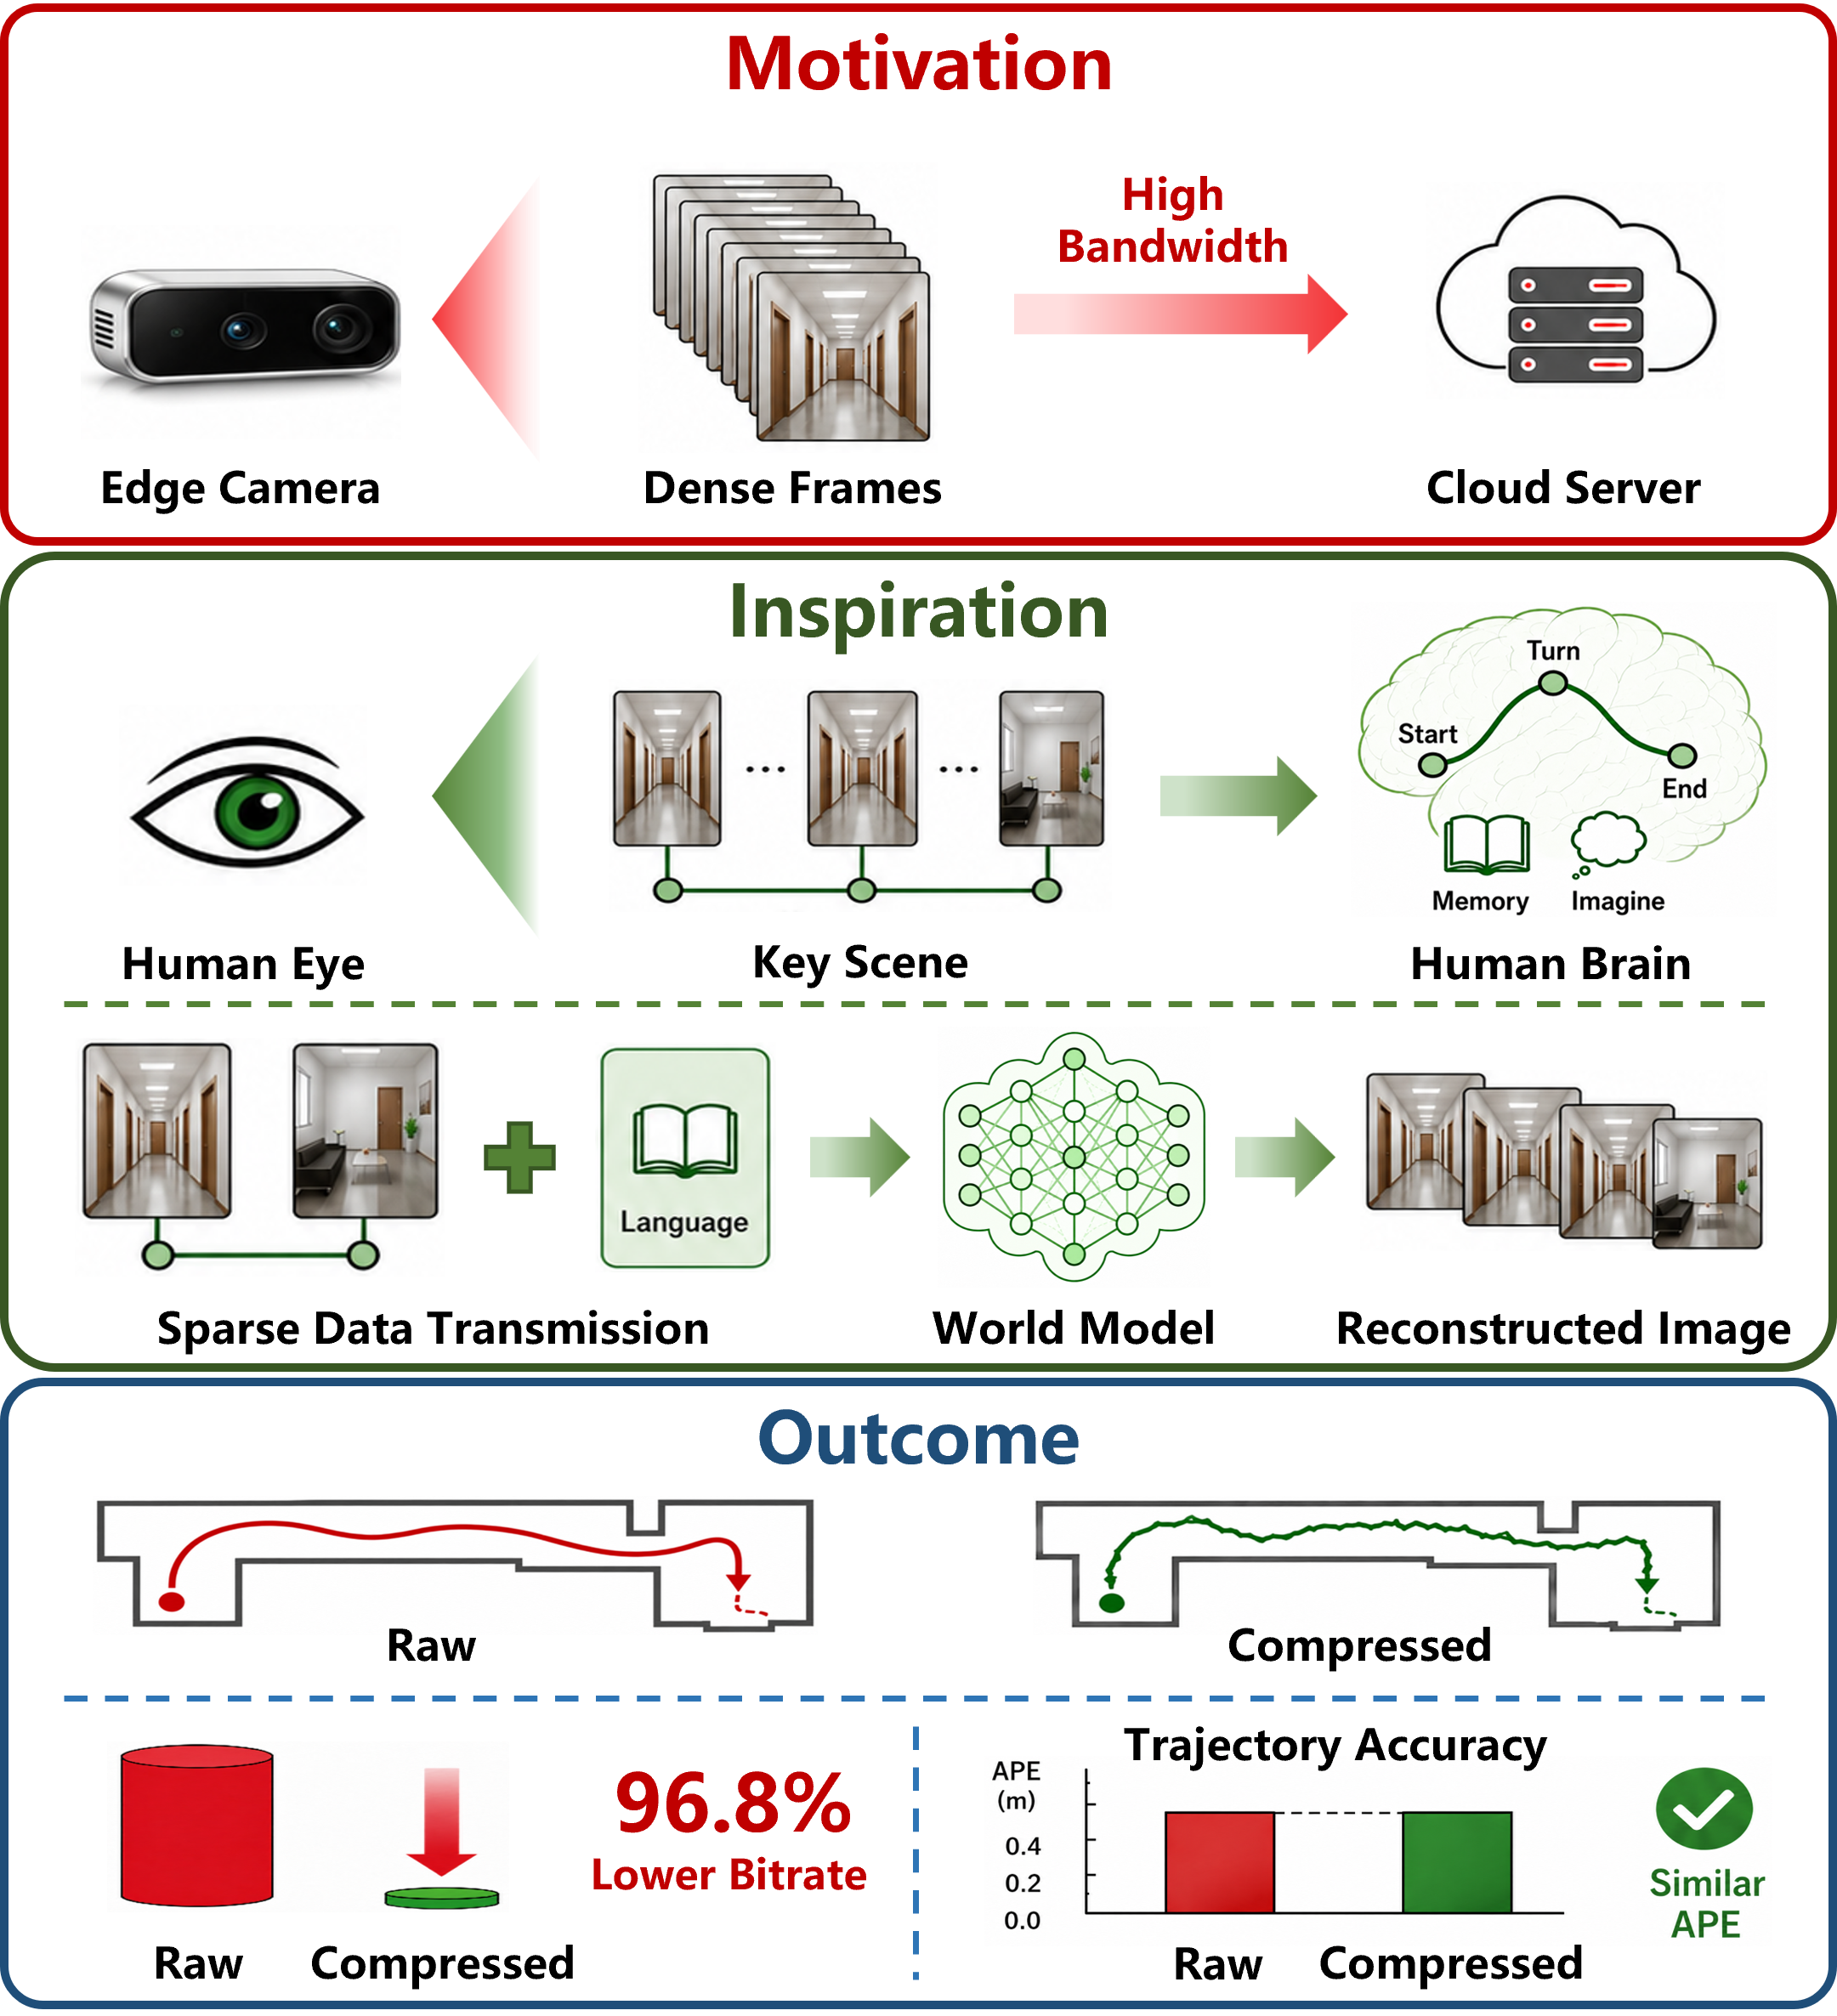
\includegraphics[width=0.95\columnwidth]{figures/fig1.png}
\caption{Motivation of human-inspired visual memory coding for edge--cloud VSLAM. Dense visual transmission requires high bandwidth, whereas the proposed memory-based formulation transmits sparse visual novelty anchors and compact language memory for task-oriented reconstruction.}
\label{fig:concept}
\end{figure}

Existing image and video compression standards reduce this burden by exploiting spatial and temporal pixel redundancy. Although such codecs are highly effective for human viewing, their rate--distortion objectives are not directly aligned with VSLAM. For VSLAM, utility depends less on pixel-identical reconstruction than on feature repeatability, geometric continuity, trackable visual textures, and temporally consistent camera motion. Under aggressive compression, images that remain visually acceptable to humans may lose stable local features, introduce temporal artifacts, or distort geometric cues used by downstream pose estimation. Therefore, edge--cloud VSLAM transmission should not be treated merely as conventional video delivery, but as a task-oriented visual transmission problem in which the transmitted representation is formulated and evaluated by downstream VSLAM utility. Fig.~\ref{fig:concept} conceptually illustrates this motivation, while the quantitative compression and trajectory tradeoffs are reported in Section~\ref{sec:experiments}.

As a design analogy, this paper is motivated by a human-inspired view of visual memory. When navigating through an environment, humans need not retain every pixel of every frame; they often recall sparse key scenes, landmarks, motion transitions, and high-level semantic impressions. This analogy does not provide a biological model, but it suggests an engineering representation for edge--cloud VSLAM image transmission: a dense visual stream can be represented by sparse image--text visual memories. In this representation, boundary frames provide geometric anchors, motion transitions and visual novelty anchors indicate what should be retained, language memory provides compact high-level conditions, and a cloud-side generative model reconstructs task-usable visual continuity.

Based on this formulation, we propose \emph{HVM-Codec}, a human-inspired image--text visual memory coding framework for edge--cloud VSLAM. For each visual memory unit, the edge transmits boundary frames as geometric constraints and constructs compact language memory to describe motion intent, scene priors, and reconstruction constraints. The boundary frames constrain the start and end appearance of the segment, while the language memory represents part of the omitted visual information with a lower-bit abstraction. The cloud-side image--text conditioned world-model decoder uses its learned visual prior to reconstruct task-usable intermediate frames. The reconstructed sequence is then fed into a cloud-side VSLAM backend for trajectory estimation.

The key mechanism behind HVM-Codec is the combination of three complementary information sources. First, boundary frames preserve visual and geometric constraints that are difficult to describe purely by language. Second, language memory encodes high-level motion and semantic priors with low communication cost. Third, the cloud-side world-model decoder supplies plausible intermediate visual continuity from its learned prior under the image--text constraints. In this way, dense visual transmission is reformulated as a compact image--text memory transmission problem rather than a generic video compression problem.

To make this framework practical for edge--cloud VSLAM, HVM-Codec adopts a lightweight edge-side memory encoder. Instead of running heavy online captioning or dense optical-flow networks on the edge, the encoder uses low-cost visual measurements to estimate coarse motion memory and visual novelty anchors. These cues are then converted into structured language memory through a controllable prompt vocabulary and motion-conditioned templates. In the cloud decoding stage, Low-Rank Adaptation (LoRA) produces a LoRA-tuned decoder that is biased toward navigation-style visual transitions and VSLAM-oriented reconstruction. In this work, reconstruction is evaluated primarily by downstream VSLAM trajectory accuracy using absolute pose error (APE) RMSE, while transmission reduction, edge-side motion-estimation cost, and auxiliary image-fidelity metrics are reported to characterize the tradeoffs.

The main contributions of this paper are summarized as follows:
\begin{itemize}
    \item We propose a human-inspired image--text visual memory coding framework for edge--cloud VSLAM that replaces dense frame transmission with sparse boundary frames and compact language memory.
    \item We design a lightweight edge-side visual memory encoder that selects boundary frames, extracts coarse motion memory and visual novelty cues, and converts them into compact language memory without relying on heavy online generative captioning.
    \item We develop an image--text conditioned cloud-side world-model decoder with LoRA adaptation for VSLAM-oriented reconstruction, where boundary frames and language memory jointly constrain task-usable intermediate-frame generation.
    \item We evaluate task-level edge--cloud visual transmission tradeoffs through compression and APE RMSE results, edge-side motion-estimation cost, and Base/LoRA decoder behavior with auxiliary LPIPS, SSIM, and FID metrics.
\end{itemize}

The remainder of this paper is organized as follows. Section~\ref{sec:related_work} reviews related work on edge--cloud VSLAM transmission, sparse visual memory coding for navigation, and world models for visual sequence reconstruction. Section~\ref{sec:methodology} presents the proposed HVM-Codec framework. Section~\ref{sec:experiments} reports the experimental evaluation and ablation studies. Section~\ref{sec:discussion} presents the discussion and limitations. Section~\ref{sec:conclusion} concludes the paper.
